\documentclass[12pt]{article}
\usepackage[backend=bibtex,style=numeric]{biblatex} 
\usepackage[breaklinks=true, bookmarks=false]{hyperref}

\usepackage{graphicx}

\addbibresource{references.bib} 

\title{Report for the CPS Final Project}
\author{
    Andrea Auletta \\ \texttt{andrea.auletta@studenti.unipd.it} \and
    Niccolò Zenaro \\ \texttt{niccolo.zenaro@studenti.unipd.it}
}
\begin{document}

\maketitle
\newpage
\tableofcontents
\newpage

\begin{abstract}
Modbus is a commonly used protocol in Supervisory Control And Data Acquisition (\textit{SCADA}) environments
for monitoring, control and data acquisition. Despite its wide popularity, Modbus is not secure because when it was developed and adopted ($1979$) security was not considered to be a concern in isolated Industrial Control Systems (\textit{ICS}), thus is not designed to be secure like modern IT networks.
Among the various attacks, 4 different taxonomies can be identified to facilitate formal risk analysis efforts for clarifying the nature and the scope of the security threats on Modbus systems and networks.
\end{abstract}

\section{Introduction and objectives}
\subsection{Modbus}
The Modicon Commuication Bus (\textit{Modbus}) protocolo operates in a master-slave or server-client based model. The master devices initiates the queries while the slave devices respond to all such queries.
Masters can either send a broadcast message to all the slaves or indivdually poll a specific device. 
All the experiments run in this work, like in the original paper \cite{huitsing2008attack} are focused on TCP/IP implementation, while Modbus protocol can be implemented also on top of several communication networks like serial or UDP. 

Modbus TCP messages are wrapped in TCP/IP header and transmitted over an ethernet-based Modbus network between different devices. The \textit{Modbus Slaves} listen for incoming TCP connections on port 503, that has been selected by us, and once a connection has been established the Protocol Data Unit (\textit{PDUs}) are exchanged and encapsulated in TCP messages. The protocol itself can be broken down into six sections: 
\begin{itemize}
    \item Transaction Identifier: a 2-byte field that is used to correlate request and responses; it is easily predictable due to poor randomization.
    \item Protocol identifier: a 2-byte field that for Modbus is always set to 0.
    \item Length: a 2-byte field that indicates the length of remaining bytes in the payload.
    \item Unit Identifier: 1 byte that is used to identify the specific slave at an IP address.
    \item Function Code: is a 1-byte field that indicates the action requested my master. For example, reading and writing coils, registers or holding registers.
    \item Data: this field has variable length, with values associated with the various function codes. 
\end{itemize}

\subsection{Attack identification}
In general attacks on Modbus systems and networks can exploit protocol's specifications, i.e. they are common to all Modbus systems/networks that are conform to the protocol specifications. The attack identification methodology used by the authors \cite{huitsing2008attack} involves an analysis of each protocol, that leads to four groups or threat categories: \textit{interception}, \textit{interruption}, \textit{modification}, \textit{fabrication}.
The main targets for the Modbus protocol are the master, the field device, the serial communication links and messages. Attacks were implemented based on the possibility of the system to have a Modbus sniffer and a packet injector, that also could block, modify or fabricate arbitrary Modbus messages or sequences of messages. 

Fifteen attacks that exploit TCP protocols have been recognized, and as said require access to the master device, network communication path or field device.
The most serious attacks are those that disable or bypass the master unit and seize control of field devices, this type of attacks affect the integrity and the availability of the messages or of the network; on the other hand attacks on confidentiality involve obtaining information on the network or on slave devices by simply reading messages.

\subsection{Objectives}
In this work we tried to emulate the various attacks defined by the authors, precisely we emulate one attack for each taxonomy identified in the paper. We built our own Modbus simulator with python libraries and then we produced python scripts for each attack.
More precisely, \textit{interception}, \textit{interruption}, \textit{modification} and \textit{fabrication} identified in the original paper are described and implemented as:
\begin{itemize}
    \item Interception: \textit{Passive reconnaissance} involves passively reading Modbus messages or network traffic, intercepting the messages and reading field device data.
    \item Interruption: \textit{TCP FIN flood} is an interruption attack that aims to launch spoofed TCP packets with the FIN flag set after a legitimate message from Modbus server to Modbus client, in order to close the TCP connection or cause important delays.
    \item Modification: \textit{Response Delay} involves delaying a response message so that the master receives out-of-date information from slaves, and is done sniffing and modifying field device, sending the modified packet with a delay.
    \item Fabrication: \textit{Rogue Interloper} is a sort of man-in-the-middle attack where a MITM device can sniff and fabricate messages.
\end{itemize}

\section{System setup}
This work was entirely done with python scripts, crafting master and slaves with \href{https://pymodbus.readthedocs.io/en/latest/}{\texttt{PyModbus}} and working on TCP level with \href{https://scapy.readthedocs.io/en/latest/}{\texttt{Scapy}}.
Although these are two of the most famous python labraries for dealing with TCP Modbus packets, we found out that their documentation is often incomplete and not accurate, with most of the informations difficult to retrieve. 

Wireshark was employed for sniffing the entire connection on the \texttt{Loopback interface} and on \texttt{port 503}, in order to obtain a feedback on what actually happened on our Modbus TCP network.

\section{Experiments}
In this section we describe the experiments done to emulate the attacks. We assume that the attacker knows IP address and the port where the devieces are listening. 
First of all, in all the experiments we have a master and a slave. The slave is a simple Modbus server that listens on port 503 and the master is a Modbus client that sends requests to the slave. So run the \texttt{slave.py} script on a terminal to start the server listening. In the file 
\texttt{master.py} there are three different function used to read, write coils and registers:
\begin{itemize}
    \item master\_read(): reads the data from all the registers of the slave;
    \item master\_connected(time\_wait): the master will be connected for 
    time\_wait seconds to the slave, it will read coils and will be disconnected time\_wait seconds;
    \item master\_write(): writes values in the holding registers of the slave.
\end{itemize}
One of these functions is called based on the attack type (change it in the main function of the file).
The master have to be run in a different terminal.
\subsection{Interception attack}
The goal of this attack is to intercept a sent message from the master to the slave. In the master, the function \texttt{master\_read()} is called. Before calling the master, run the \texttt{interception.py} script that will sniff the packet and print it. The attacker will listen to the network and when it found the packet with the right characteristics, it will print it.
\begin{figure}[h]
    \centering
    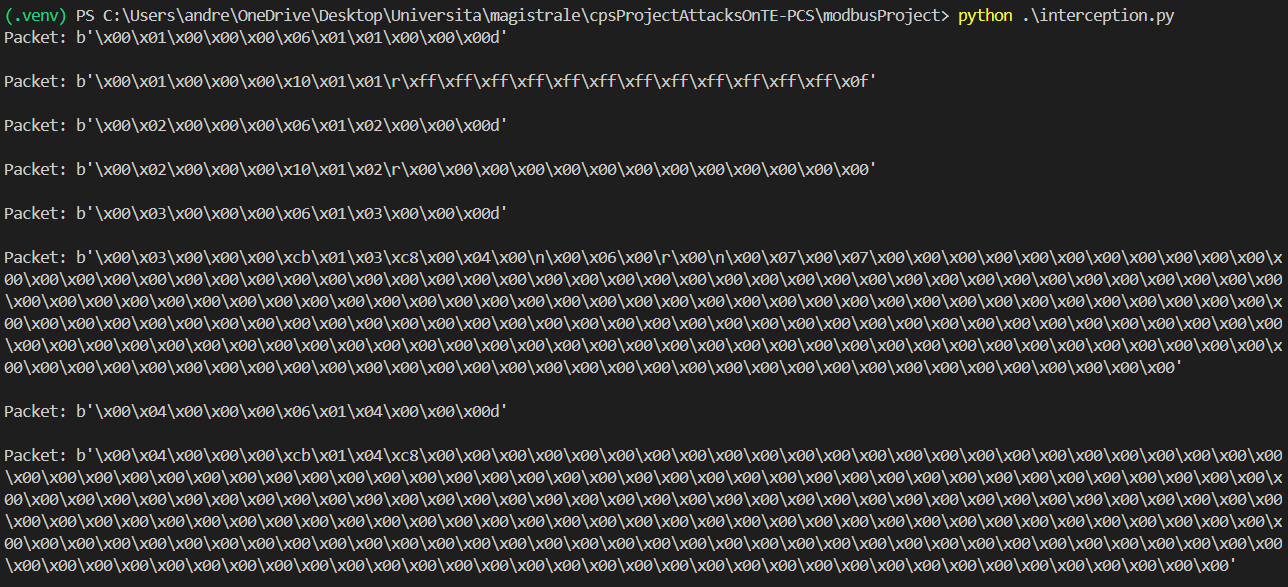
\includegraphics[width=1\textwidth]{images/InterceptionResults.png}
    \caption{Results of the interception attack}
    \label{fig:interceptionResult}
\end{figure}
In the image \ref{fig:interceptionResult} we can see that there are 4 operations requested by the master and 4 responses from the slave.
Here there is a conversion of the first packet present in the image:
\begin{enumerate}
    \item Transaction ID = x00x01 = 1;
    \item Protocol ID = x00x00 = 0;
    \item Length = x00x06 = 6;
    \item Unit ID = x01 = 1;
    \item Function Code = x01 = 1 (read coils);
    \item Data = x00x00x00;
\end{enumerate}
We found the function codes and their assignd functions in the following site \href{https://ozeki.hu/p_5873-modbus-function-codes.html}{codes}
\section{Results and Discussion}
\printbibliography 


\end{document}
